\documentclass[border=10pt]{standalone}
\usepackage{tikz}
\usetikzlibrary{hobby}
\definecolor{myred}{RGB}{190,60,45}
\definecolor{myblue}{RGB}{38,84,160}
\begin{document}
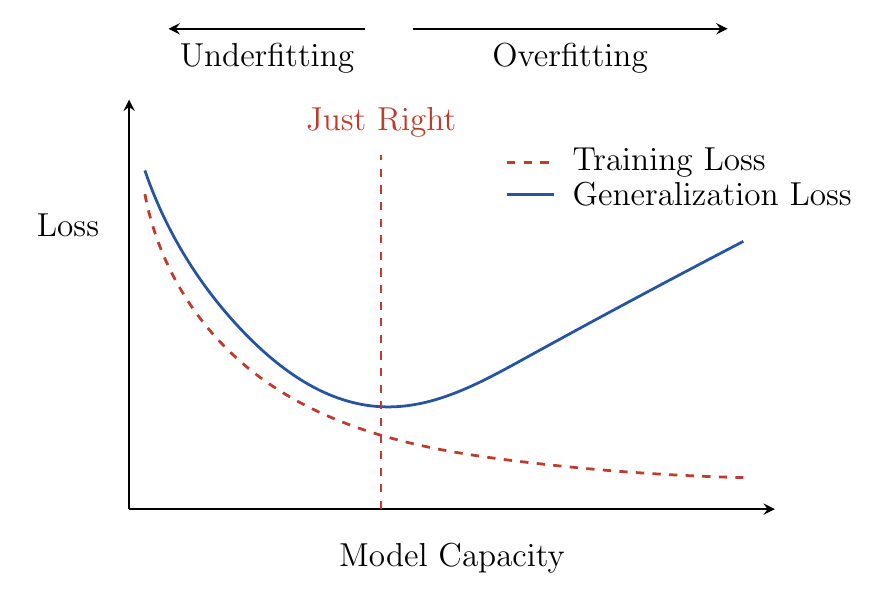
\begin{tikzpicture}[>=stealth, line width=0.8pt, font=\large]
  % 坐标轴（标签分离出去，单独摆放）
  \draw[->] (0,0) -- (8.2,0);
  \draw[->] (0,0) -- (0,5.2);
  \node[below] at (4.1,-0.3) {Model Capacity};   % x 轴下方居中
  \node[left]  at (-0.25,3.6) {Loss};             % y 轴左侧

  % 训练损失：一路降（虚线，红）
  \draw[myred, line width=1pt, dashed] (0.2,4.0)
    to[curve through={(1.5,1.8) (3,1.0) (5,0.6)}] (7.8,0.4);
  % 泛化损失：先降后升（实线，蓝）
  \draw[myblue, line width=1pt] (0.2,4.3)
    to[curve through={(1.5,2.2) (3.2,1.3) (5,1.9)}] (7.8,3.4);

  % 顶部区域箭头
  \draw[<-] (0.5,6.1) -- (3.0,6.1);
  \node[below] at (1.75,6.05) {Underfitting};
  \draw[->] (3.6,6.1) -- (7.6,6.1);
  \node[below] at (5.6,6.05) {Overfitting};

  % Just Right 竖虚线
  \draw[myred, dashed] (3.2,0) -- (3.2,4.5);
  \node[myred, above] at (3.2,4.6) {Just Right};

  % 图例
  \draw[myred, line width=1pt, dashed] (4.8,4.4) -- (5.4,4.4);
  \node[right] at (5.5,4.4) {Training Loss};
  \draw[myblue, line width=1pt] (4.8,4.0) -- (5.4,4.0);
  \node[right] at (5.5,4.0) {Generalization Loss};
\end{tikzpicture}
\end{document}